\documentclass[a4paper,12pt]{article}

% Pacchetti necessari
\usepackage[utf8]{inputenc}
\usepackage{graphicx}
\usepackage{amsmath}
\usepackage{hyperref}
\usepackage{listings}
\usepackage{float}
\usepackage{caption}
\usepackage{subcaption}
\usepackage{booktabs}
\usepackage{xcolor}
\usepackage{geometry}

% Definizione dei colori per il codice
\definecolor{codebg}{rgb}{0.95, 0.95, 0.95}
\definecolor{codecmnt}{rgb}{0.25, 0.5, 0.35} % Commenti più scuri
\definecolor{codekw}{rgb}{0.2, 0.4, 0.8} % Parole chiave con un blu meno brillante
\definecolor{codeid}{rgb}{0.6, 0.4, 0.8} % Identificatori meno sgargianti
\definecolor{codegray}{rgb}{0.4, 0.4, 0.4} % Numeri di riga meno intensi

% Stile personalizzato per il codice
\lstdefinestyle{mystyle}{
    backgroundcolor=\color{codebg},   
    commentstyle=\color{codecmnt},
    keywordstyle=\color{codekw},
    numberstyle=\tiny\color{codegray},
    stringstyle=\color{codeid},
    basicstyle=\ttfamily\footnotesize,
    breaklines=true,
    captionpos=b,                    
    keepspaces=true,                 
    numbers=left,                    
    numbersep=5pt,                  
    showspaces=false,                
    showstringspaces=false,
    tabsize=2
}

\lstset{style=mystyle}

% Impostazione dei link senza bordo
\hypersetup{
    colorlinks=true,
    linkcolor=black,
    filecolor=black,      
    urlcolor=blue,
    pdfborder={0 0 0}, % Elimina il contorno dei link
}

% Impostazione delle dimensioni della pagina
\geometry{
    a4paper, % Formato della pagina
    left=2.5cm, % Margine sinistro
    right=2.5cm, % Margine destro
    top=3cm, % Margine superiore
    bottom=3cm, % Margine inferiore
}

% Titolo del documento
\title{
    \vspace{-2cm} % Spazio per allineare correttamente l'intestazione
    \textbf{\Large Università degli Studi di Palermo} \\
    \vspace{0.3cm}
    \textbf{\Large Corso di Laurea in Informatica} \\
    \vspace{1cm}
    \textbf{\Large Esame di ``Laboratorio di Algoritmi''} \\
    \vspace{0.5cm}
    \textbf{\Large Relazione della prova pratica} \\
    \vspace{2cm}
    \textbf{Habasescu Alin Marian} \\
    \vspace{0.5cm}
    \textbf{\Large Soluzione prova pratica} \\
    \vspace{1cm}
}

\date{\normalsize Data di consegna: \today} % Data del documento

\begin{document}

\maketitle % Genera il titolo

\tableofcontents % Genera l'indice
\clearpage

\section{Soluzione proposta}
Il progetto richiede la minimizzazione della perdita d'acqua nel trasporto tra acquedotti, 
modellando la rete idrica come un grafo pesato dove i nodi rappresentano gli acquedotti 
e i lati bidirezionali rappresentano le tubazioni con un determinato livello di perdita 
d'acqua misurata in millilitri al secondo. \\

Il problema principale sta nel voler calcolare i millilitri al secondo che vengono persi 
lungo una sequenza di tubi, da un certo acquedoto S ad un
altro acquedoto T, individuando la minor perdita possibile.\\

Per risolvere il problema, ho scelto di applicare l'algoritmo di Dijkstra, 
che è particolarmente adatto a determinare il percorso con costo minimo in termini di peso,
da un vertice S detto ``sorgente'' ad un vertice T detto ``destinazione'', 
purché i pesi degli archi siano non negativi.\\

\subsection{Algoritmi e codice utilizzati}
Durante lo svolgimento del corso, ho creato una repository GitHub in cui ho raccolto 
diverse implementazioni di algoritmi e strutture dati. Questa raccolta mi è stata 
particolarmente utile per il completamento del progetto, in cui ho riutilizzato e 
adattato alcune delle implementazioni, tra cui:

\begin{itemize}
    \item \texttt{WeightedGraph}, una classe per la gestione di grafi pesati, 
    implementata sia tramite liste di adiacenza, che matrici di adiacenza.
    \item L'algoritmo di \textbf{Dijkstra} che calcola il percorso minimo in un 
    grafo pesato, è stato implementato nella classe \texttt{GraphAlgorithms}.
    \item \texttt{Heap}, una classe per la gestione della coda di priorità, utilizzata 
    all'interno dell'algoritmo di Dijkstra per mantenere traccia dei nodi da processare.
\end{itemize}

Il codice sorgente completo è disponibile al seguente link:

\begin{quote}
    \url{https://github.com/H-Alin02/DSA-in-cpp}
\end{quote}

All'interno del progetto, ho sviluppato un file \texttt{ProvaPratica.cpp}, che contiene il 
\textit{main} del programma e gestisce l'interazione con i file di input e output. 
In particolare, utilizzo la funzione 
\texttt{GraphType getInputData (string path, int\& source, int\& destination)} 
per caricare i dati da un file di testo.

Il file di input contiene:
\begin{itemize}
    \item Il numero $n$ di acquedotti ($2 \leq n \leq 200$);
    \item Il numero $m$ di tubi ($0 \leq m \leq 5000$);
    \item Gli acquedotti $S$ e $T$ di partenza e arrivo ($1 \leq S, T < n$);
    \item Le successive $m$ righe contengono tre valori: due numeri di acquedotti collegati 
    da un tubo e la perdita d'acqua $p$ (in millilitri al secondo), con $0 \leq p \leq 1000$, 
    del tubo bidirezionale che li connette.
\end{itemize}

Il file di output conterrà la perdita d'acqua minima, in millilitri al secondo, tra gli acquedotti $S$ e $T$.

Di seguito, mostro il codice del \textit{main} e della funzione \texttt{getInputData}.

\begin{lstlisting}[language=c++, label=main]
int main() {
    int source, destination, result;

    // Crea 3 grafi di testing e li inizializza con i dati di input
    for (int i = 1; i <= 3; i++) {
        // Crea un grafo pesato rappresentato da liste di adiacenza 
        // e lo inizializza con i dati di input
        GraphType graph = getInputData("inputs/input" + to_string(i) + ".txt", source, destination);
        cout << "Grafo " << i << ": " << endl;
        graph.print();

        // Applica l'algoritmo di Dijkstra e stampa a console la soluzione
        result = GraphAlgorithms<int, GraphType>::dijkstra(source, destination, graph);
        cout << "Dijkstra da " << source << " a " << destination << ": " << result << " ml/s\n\n";

        // Scrivi il risultato su un file di output
        ofstream outfile("outputs/output" + to_string(i) + ".txt");
        if (!outfile) {
            cerr << "Errore nell'apertura del file di output" << endl;
            return 1;
        }

        outfile << "Dijkstra da " << source << " a " << destination << ": " << result << " ml/s" << endl;

        // Chiudi il file di output
        outfile.close();
    }

    return 0;
}
\end{lstlisting}

\clearpage

\begin{lstlisting}[language=c++, label=getInputData]
GraphType getInputData(string path, int& source, int& destination) {
    int acquedotti, tubi;

    // Apre il file di input
    ifstream infile(path); 
    if (!infile) {
        cerr << "Errore nell'apertura del file di input" << endl;
        exit(1);
    }

    // Legge il numero di acquedotti, tubi, e i nodi di partenza e destinazione
    infile >> acquedotti >> tubi >> source >> destination;

    // Controlla che i valori siano validi
    if (source < 0 || source >= acquedotti || destination < 0 || destination >= acquedotti) {
        throw out_of_range("Nodo di partenza o destinazione non valido");
    }
    if (acquedotti < 2 || acquedotti > 200 || tubi < 0 || tubi > 5000) {
        throw out_of_range("Numero di acquedotti o tubi non valido");
    }

    // Crea il grafo pesato
    GraphType graph(acquedotti);

    // Aggiunge i tubi al grafo
    int x, y;
    double z;
    for (int i = 0; i < tubi; ++i) {
        infile >> x >> y >> z;
        if (z < 0 || z > 1000) {
            throw out_of_range("Perdita non valida");
        }
        graph.insert(x, y, z); // Inserisce l'arco pesato
    }

    infile.close();

    return graph;
}
\end{lstlisting}

\clearpage

\subsection{Algoritmo di Dijkstra}

L'algoritmo di Dijkstra per il calcolo del percorso minimo è riportato di seguito:  

\begin{lstlisting}[language=c++, label=Dijkstra]
    // Dijkstra implementation to find the shortest path from start to destination
    static int dijkstra(int start, int end, const GraphType& graph) {
        int nodes = graph.getVertices();

        if (start < 0 || start >= nodes || end < 0 || end >= nodes) {
            throw out_of_range("Invalid start or end node");
        }

        // Priority queue to select the node with the smallest distance
        Heap<pair<T, double>> pq(
            [](const pair<T, double>& a, const pair<T, double>& b) {
            return a.second < b.second;
        }, true);

        // Initialize distances to infinity
        vector<double> dist(nodes, numeric_limits<double>::infinity());
        dist[start] = 0;
        pq.push({start, 0});

        while (!pq.empty()) {
            int u = pq.top().first; 
            int u_dist = pq.top().second;
            pq.pop();

            if (u == end)
                return u_dist;

            for (const auto &neighbor : graph.getEdges(u)) {
                int v = neighbor.first.second;
                double weight = neighbor.second;

                if (dist[v] > u_dist + weight) {
                    dist[v] = u_dist + weight;
                    pq.push({v, dist[v]});
                }
            }
        }

        return -1;
    }


\end{lstlisting}

\clearpage

\section{Correttezza dell'algoritmo}

Analiziamo ora la correttezza dell' implementazione dell'algoritmo di Dijkstra 
confrontandolo con il suo Pseudocodice originale: 

\begin{figure}[h!]
    \centering
    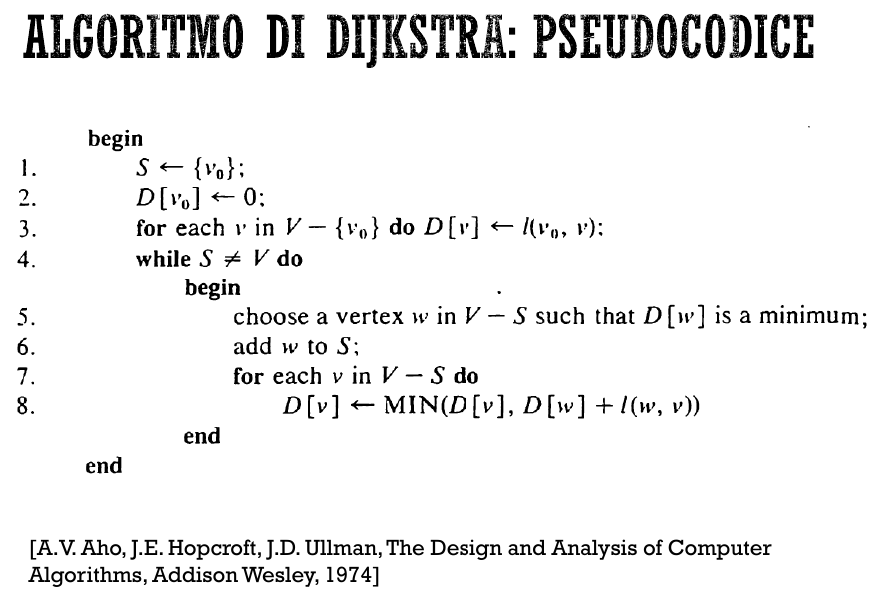
\includegraphics[width=0.7\textwidth]{Images/DijkstraPseudoCode.png}
    \caption{Pseudocodice dell'algoritmo di Dijkstra.}\label{fig:Pseudocodice Dijkstra}
\end{figure}


\begin{enumerate}
    \item \textbf{Inizializzazione del set S e del vettore dist}: Nell'implementazione, 
    il set S viene implicitamente gestito attraverso l'uso di una coda a priorità 
    (implementata con un Min-Heap).
    Se un nodo è estratto dalla coda significa che il percorso minimo per quel nodo è già
    stato trovato. Il vettore ``dist'' viene inizializzato con infinito per 
    tutti i nodi, tranne il nodo di partenza, il cui costo è impostato a 0.

    \item \textbf{Aggiornamento delle Distanze}: Durante l'iterazione, se viene trovato un 
    percorso più breve verso un nodo, la distanza viene aggiornata e il nodo viene 
    reinserito nella coda di priorità con la nuova distanza.
    Questo passaggio viene implementato con la condizione \texttt{dist[v] > u\_dist + weight},
    che aggiorna le distanze e aggiunge il nodo $v$ alla coda di priorità con la nuova distanza.

    \item \textbf{Condizione di Terminazione}: Nello pseudocodice l'algoritmo continua fino a 
    quando tutti i nodi non sono stati elaborati (cioe $S = V$), nell'implementazione l'algoritmo
    si interrompe non appena viene trovato il nodo di destinazione 
\end{enumerate}

\clearpage

\section{Alcuni esempi di esecuzione}
Di seguito vengono riportati alcuni esempi di esecuzione dell'algoritmo su piccoli grafi.

\subsection{Esempio 1}
\begin{itemize}
    \item \textbf{Input}: 5 acquedotti, 7 tubazioni, partenza da S=0, arrivo a T=4.  
    \item \textbf{Output}: La minima perdita da 0 a 4 è $9ml/s$.
\end{itemize}

\begin{figure}[h!]
    \centering
    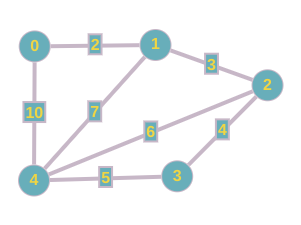
\includegraphics[width=0.4\textwidth]{Images/graph1.png}
    \caption{Grafo 1.}\label{fig:grafo1}
\end{figure}

\begin{table}[H]
    \centering
    \begin{tabular}{cccccccc}
        \toprule
        \textbf{Iteration} & \textbf{S} & \textbf{w} & \textbf{D[w]} &
        \textbf{D[1]} & \textbf{D[2]} & \textbf{D[3]} & \textbf{D[4]} \\
        \midrule
        Initial & {0} & $-$ & $-$ & 2 & +$\infty$ & +$\infty$ & 10 \\
        1 & {0,1} & 1 & 2 & 2 & 5 & +$\infty$ & 9 \\
        2 & {0,1,2} & 2 & 5 & 2 & 5 & 9 & 9 \\
        3 & {0,1,2,3} & 3 & 9 & 2 & 5 & 9 & 9 \\
        4 & All & 4 & 9 & 2 & 5 & 9 & 9 \\
        \bottomrule
    \end{tabular}
    \caption{Esecuzione del algoritmo di Dijkstra per il nodo 0 sul grafo 1}\label{tab:Tgrafo1}
\end{table}

\clearpage
\subsection{Esempio 2}
\begin{itemize}
    \item \textbf{Input}: 7 acquedotti, 8 tubazioni, partenza da S=0, arrivo a T=6.
    
    \item \textbf{Output}: La minima perdita da 0 a 6 è $19ml/s$.
\end{itemize}

\begin{figure}[h!]
    \centering
    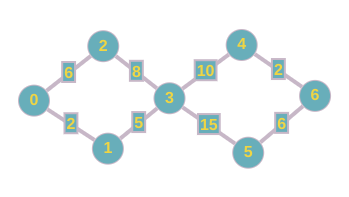
\includegraphics[width=0.4\textwidth]{Images/graph2.png}
    \caption{Grafo 2.}\label{fig:grafo2}
\end{figure}

\begin{table}[H]
    \centering
    \begin{tabular}{cccccccccc}
        \toprule
        \textbf{Iteration} & \textbf{S} & \textbf{w} & \textbf{D[w]} &
        \textbf{D[1]} & \textbf{D[2]} & \textbf{D[3]} & \textbf{D[4]} &
        \textbf{D[5]} & \textbf{D[6]} \\
        \midrule
        Initial & 0 & $-$ & $-$ & 2 & 6 & +$\infty$ & +$\infty$ & +$\infty$ & +$\infty$ \\
        1 & {0,1} & 1 & 2 & 2 & 6 & 7 & +$\infty$ & +$\infty$ & +$\infty$ \\
        2 & {0,1,2} & 2 & 6 & 2 & 6 & 7 & +$\infty$ & +$\infty$ & +$\infty$ \\
        3 & {0,1,2,3} & 3 & 7 & 2 & 6 & 7 & 17 & 22 & +$\infty$ \\
        4 & {0,1,2,3,4} & 4 & 17 & 2 & 6 & 7 & 17 & 22 & 19 \\
        5 & All & 6 & 19 & 2 & 6 & 7 & 17 & 22 & 19 \\
        \bottomrule
    \end{tabular}
    \caption{Esecuzione del algoritmo di Dijkstra per il nodo 0 sul grafo 2}
\end{table}

\clearpage
\subsection{Esempio 3}
\begin{itemize}
    \item \textbf{Input}: 9 acquedotti, 14 tubazioni, partenza da S=0, arrivo a T=8.
    \item \textbf{Output}: La minima perdita da 0 a 8 è $14ml/s$.
\end{itemize}

\begin{figure}[h!]
    \centering
    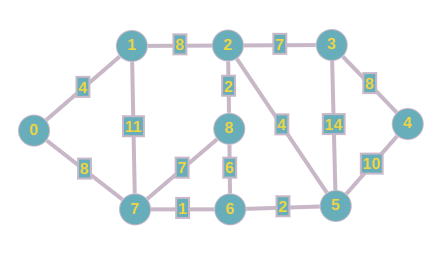
\includegraphics[width=0.4\textwidth]{Images/graph3.png}
    \caption{Grafo 3.}\label{fig:grafo3}
\end{figure}

\begin{table}[H]
    \centering
    \resizebox{\textwidth}{!}{ % Ridimensiona la tabella alla larghezza del testo
    \begin{tabular}{cccccccccccc}
        \toprule
        \textbf{Iteration} & \textbf{S} & \textbf{w} & \textbf{D[w]} & 
        \textbf{D[1]} & \textbf{D[2]} & \textbf{D[3]} & \textbf{D[4]} & 
        \textbf{D[5]} & \textbf{D[6]} & \textbf{D[7]} & \textbf{D[8]} \\
        \midrule
        Initial & 0 & $-$ & $-$ & 4 & +$\infty$ & +$\infty$ & +$\infty$ & +$\infty$ & +$\infty$ & 8 & +$\infty$ \\
        1 & {0,1} & 1 & 4 & 4 & 12 & +$\infty$ & +$\infty$ & +$\infty$ & +$\infty$ & 8 & +$\infty$ \\
        2 & {0,1,7} & 7 & 8 & 4 & 12 & +$\infty$ & +$\infty$ & +$\infty$ & 9 & 8 & 15 \\
        3 & {0,1,7,6} & 6 & 9 & 4 & 12 & +$\infty$ & +$\infty$ & 11 & 9 & 8 & 15 \\
        4 & {0,1,7,6,5} & 5 & 11 & 4 & 12 & 25 & 21& 11 & 9 & 8 & 15 \\
        5 & {0,1,7,6,5,2} & 2 & 12 & 4 & 12 & 19 & 21& 11 & 9 & 8 & 14 \\
        6 & {0,1,7,6,5,2,8} & 8 & 14 & 4 & 12 & 19 & 21& 11 & 9 & 8 & 14 \\
        7 & {0,1,7,6,5,2,8,3} & 3 & 19 & 4 & 12 & 19 & 21& 11 & 9 & 8 & 14 \\
        8 & All & 4 & 21 & 4 & 12 & 19 & 21& 11 & 9 & 8 & 14 \\
    \end{tabular}
    }
    \caption{Esecuzione dell'algoritmo di Dijkstra per il nodo 0 sul grafo 3.}
\end{table}

\clearpage

\section{Complessità di tempo e spazio}

La complessità temporale dell'algoritmo di Dijkstra dipende dall'implementazione della 
coda a priorità, che in questo caso è realizzata tramite un \textbf{heap binario}, 
e dal numero di vertici ($V$) e archi ($E$) del grafo.

\begin{enumerate} 
    \item \textbf{Operazioni sulla coda di priorità}: 
    \begin{itemize} 
        \item \textbf{Inserimento}: l'inserimento di un nuovo elemento 
        nell'heap binario ha un costo di $\mathcal{O}(\log V)$, poiché è 
        necessario mantenere l'ordinamento della struttura. 
        \item \textbf{Estrazione del minimo}: l'estrazione del nodo con 
        la distanza minima ha una complessità di $\mathcal{O}(\log V)$, 
        in quanto anche in questo caso l'heap deve essere riorganizzato per 
        preservare la proprietà di ordinamento. 
    \end{itemize}

    \item \textbf{Esplorazione del grafo}:
    \begin{itemize}
        \item L'algoritmo di Dijkstra visita ogni nodo una sola volta, 
        eseguendo al massimo $V$ operazioni di estrazione (\textit{pop}) dalla coda 
        a priorità. Inoltre, esplora ogni arco del grafo esattamente una volta per 
        verificare se la distanza dei nodi adiacenti deve essere aggiornata.
        \item Ogni aggiornamento di distanza richiede un'inserzione o un'operazione 
        di riduzione della chiave nella coda a priorità, operazioni che entrambe 
        hanno una complessità di $\mathcal{O}(\log V)$. Considerando che ci sono $E$ 
        archi, in totale si eseguono al massimo $E$ operazioni di inserimento o 
        aggiornamento nell'heap.
    \end{itemize}
\end{enumerate}

In sintesi, la complessità temporale complessiva dell'algoritmo di Dijkstra, 
utilizzando un heap binario, è $\mathcal{O}(E \log V + V \log V)$, che si può 
esprimere come $\mathcal{O}((E + V) \log V)$.\\

\textbf{Complessità spaziale}: Il grafo può essere rappresentato mediante una lista di 
adiacenza, occupando spazio $\mathcal{O}(V + E)$, oppure tramite matrice di adicenza, 
occupando spazio $\mathcal{O}(V^2)$. 
La coda a priorità contiene al massimo $V$ elementi, quindi anch'essa 
richiede spazio $\mathcal{O}(V)$. 
Pertanto, la complessità spaziale complessiva dipende dal tipo di rappresentazione 
che si sceglie di usare. 

Considerando i limiti sui dati di input (con $n \leq 200$ acquedotti e $m \leq 5000$ tubi), 
sarebbe consigliabile utilizzare la rappresentazione 
tramite lista di adiacenza.

\clearpage

\section{Strutture dati utilizzate}
Per rappresentare il grafo, ho utilizzato due possibili rappresentazioni:
\begin{itemize}
    \item \textbf{Lista di adiacenza}: Questa struttura è stata utilizzata per ridurre lo 
    spazio necessario per grafi sparsi. Permette di memorizzare efficientemente i vicini di 
    ogni nodo e le loro perdite associate.
    \item \textbf{Matrice di adiacenza}: Utilizzata per rappresentare grafi più densi, anche 
    se meno efficiente in termini di spazio.
\end{itemize}

Per la gestione della selezione del nodo successivo con la minima distanza, è stata 
utilizzata una \textbf{coda con priorità} implementata come min-heap, che permette 
l'accesso al nodo con il peso minore in tempo $O(\log V)$. Questo garantisce che 
l'algoritmo funzioni in modo efficiente anche con un numero elevato di nodi.
\end{document}
